%versi 2 (8-10-2016)-pppppppppppppp;
\chapter{Analisis}
\label{chap:analisis}
\setcounter{secnumdepth}{3}

\paragraph{} Pengumpulan data dalam skripsi ini dilakukan dengan cara studi pustaka untuk mempelajari cara pengembangan perangkat lunak menggunakan \textit{Framework} BlueTape yang berbasis CodeIgniter. Selain itu juga dipelajari \textit{library-library} pembantunya diantara lain : PHPExcel , Google OAuth dan ZurbFoundation. Tujuan studi pustaka ini untuk memahami secara rinci cara-cara untuk menambahkan layanan berbentuk modul ke dalam BlueTape dan membangun layanan tersebut menggunakan \textit{library-library} yang disebutkan sebelum ini.

\section{Analisis Sistem Kini}
\paragraph{} Aplikasi \textit{Blue Tape} adalah perangkat lunak \textit{open source} sederhana yang memiliki tujuan utama untuk mengubah berbagai pekerjaan \textit{paper-based} di FTIS UNPAR menjadi \textit{paperless}. Selain itu perangkat lunak ini memiliki beberapa kegunaan lainnya seperti mengautentikasi mahasiswa dan staf UNPAR via OAuth 2.0 ke Google (layanan OAuth ke Google ini juga dapat digunakan untuk menentukan hak akses yang bisa dilihat dari email pengguna) dan \textit{Pilot Project} untuk permohonan transkrip ke Tata Usaha . Aplikasi ini merupakan aplikasi berbasis web dengan memanfaatkan \textit{Codeigniter} dan \textit{Zurb Foundation}. 
\newline
\begin{figure} [H]
	\centering  
	\frame{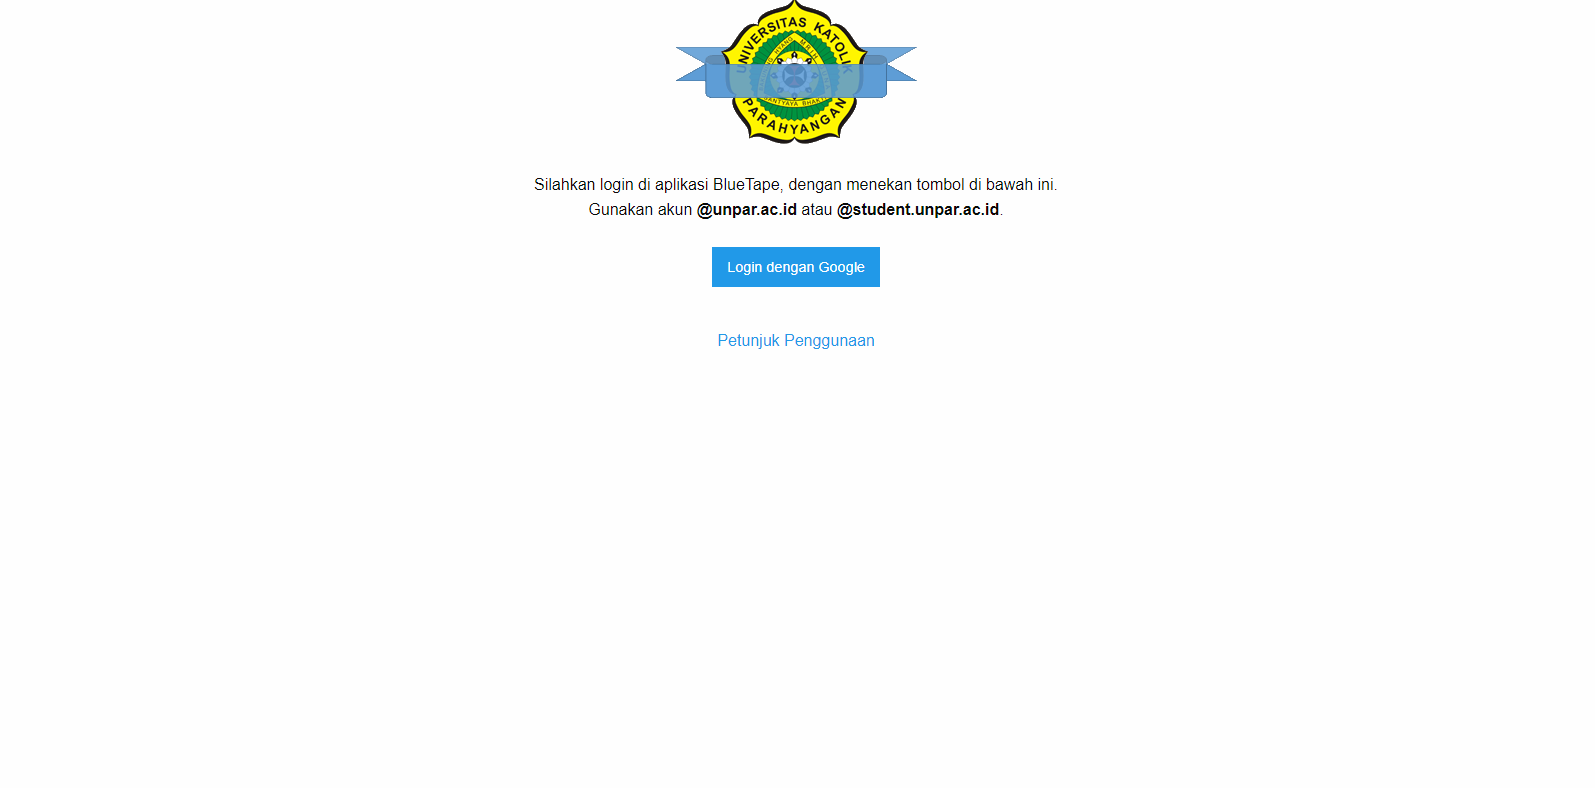
\includegraphics[scale=0.4]{halamanUtama.png}}
	\caption[Halaman Utama BlueTape Untuk Login dan Membuka Petunjuk Penggunaan]{Halaman Utama BlueTape Untuk Login dan Membuka Petunjuk Penggunaan} 
	\label{fig:flow-chart-CodeIgniter} 
\end{figure}
Perangkat lunak \textit{Blue Tape} ini didesain sebagai \textit{framework} yang terdiri dari beberapa layanan yang dipisahkan ke dalam modul-modul. Pemisahan layanan ke dalam modul-modul dibuat dengan tujuan agar pemeliharan perangkat lunak lebih mudah dan juga mempermudah cara untuk menambahkan layanan baru ke dalam BlueTape. Sudah ada layanan yang aktif di BlueTape saat ini yaitu \textit{Transcript Request / Manage} yang memiliki fungsi untuk melakukan permohonan serta pencetakan transkrip mahasiswa.

\subsection{\textit{Transcript Request / Manage}}
\paragraph{} Modul \textit{Transcript Request/Manage} merupakan salah satu dari dua modul yang sudah aktif di BlueTape ketika skripsi ini ditulis. Modul ini memiliki fungsi utama sebagai alat bagi mahasiswa untuk memohon pencetakan transkrip ke Tata Usaha dengan tampilan seperti di bawah ini :
\begin{figure} [H]
	\centering  
	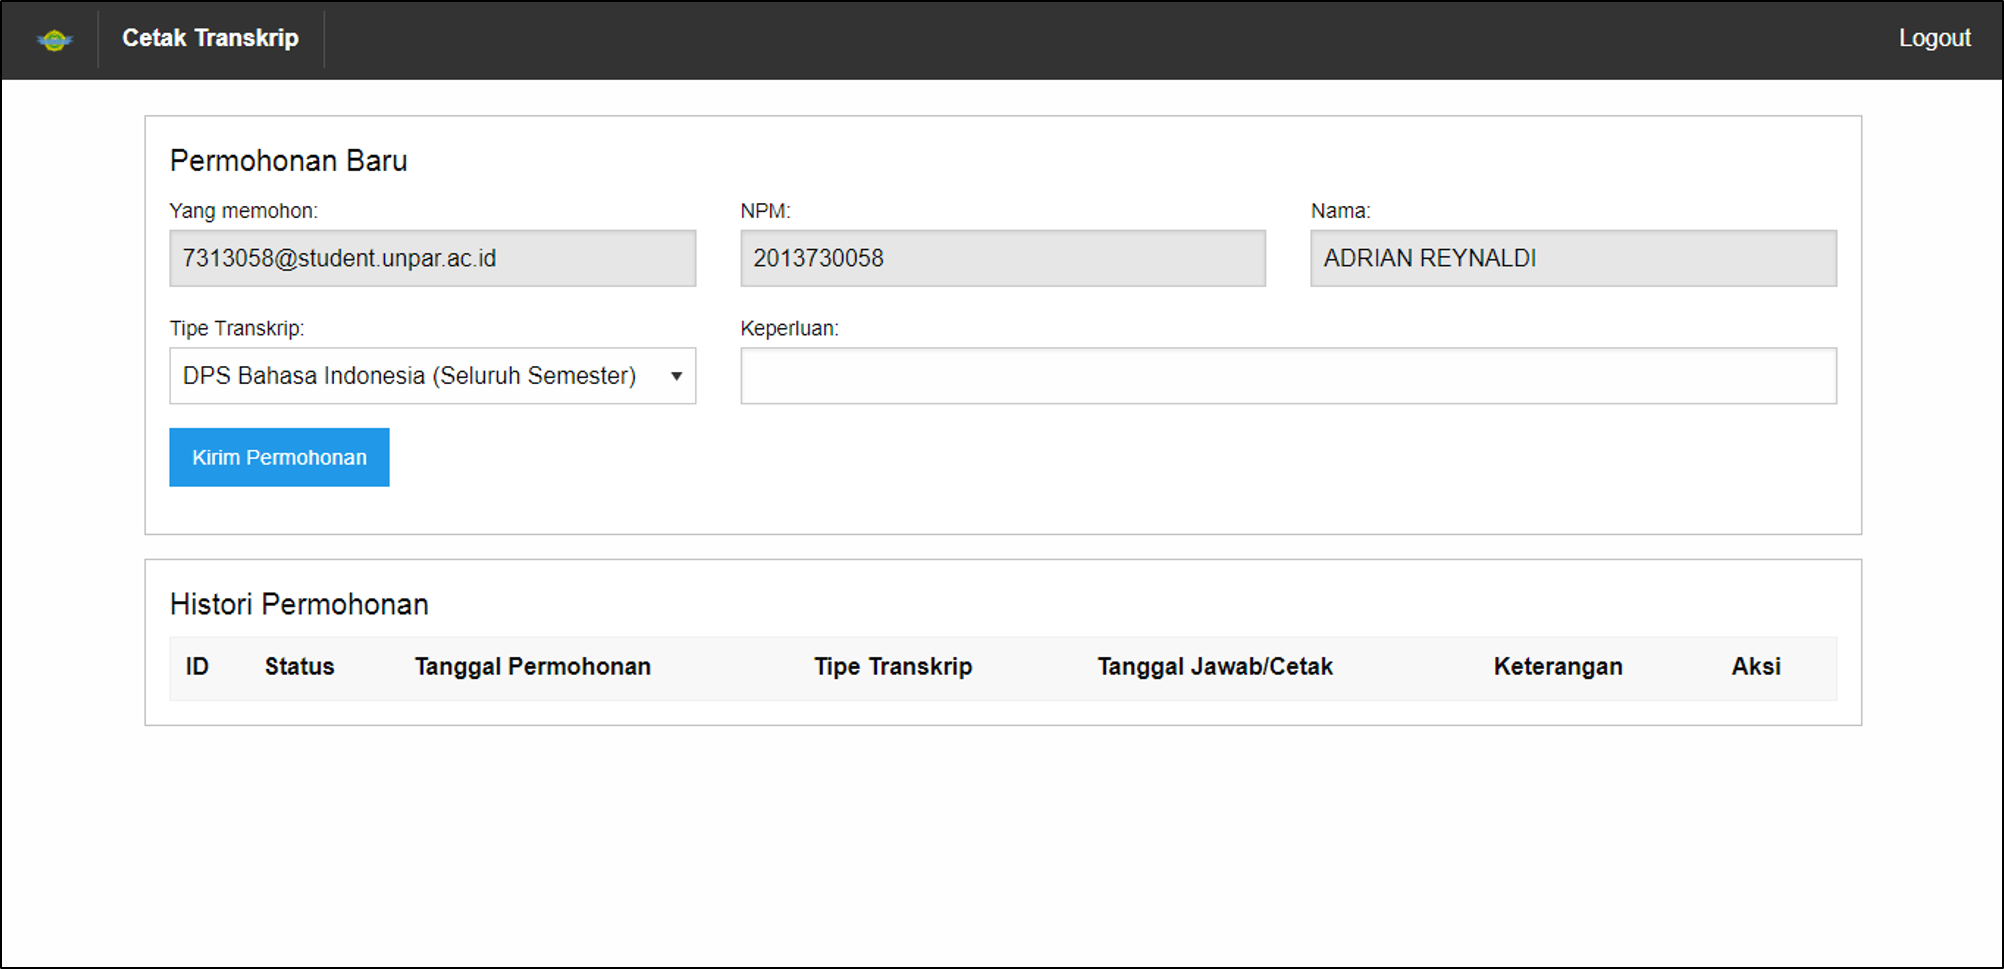
\includegraphics[scale=0.48]{cetakTranskrip.png}
	\caption[Tampilan Cetak Transkrip]{Tampilan Cetak Transkrip} 
\end{figure}
\begin{figure} [H]
	\centering  
	\frame{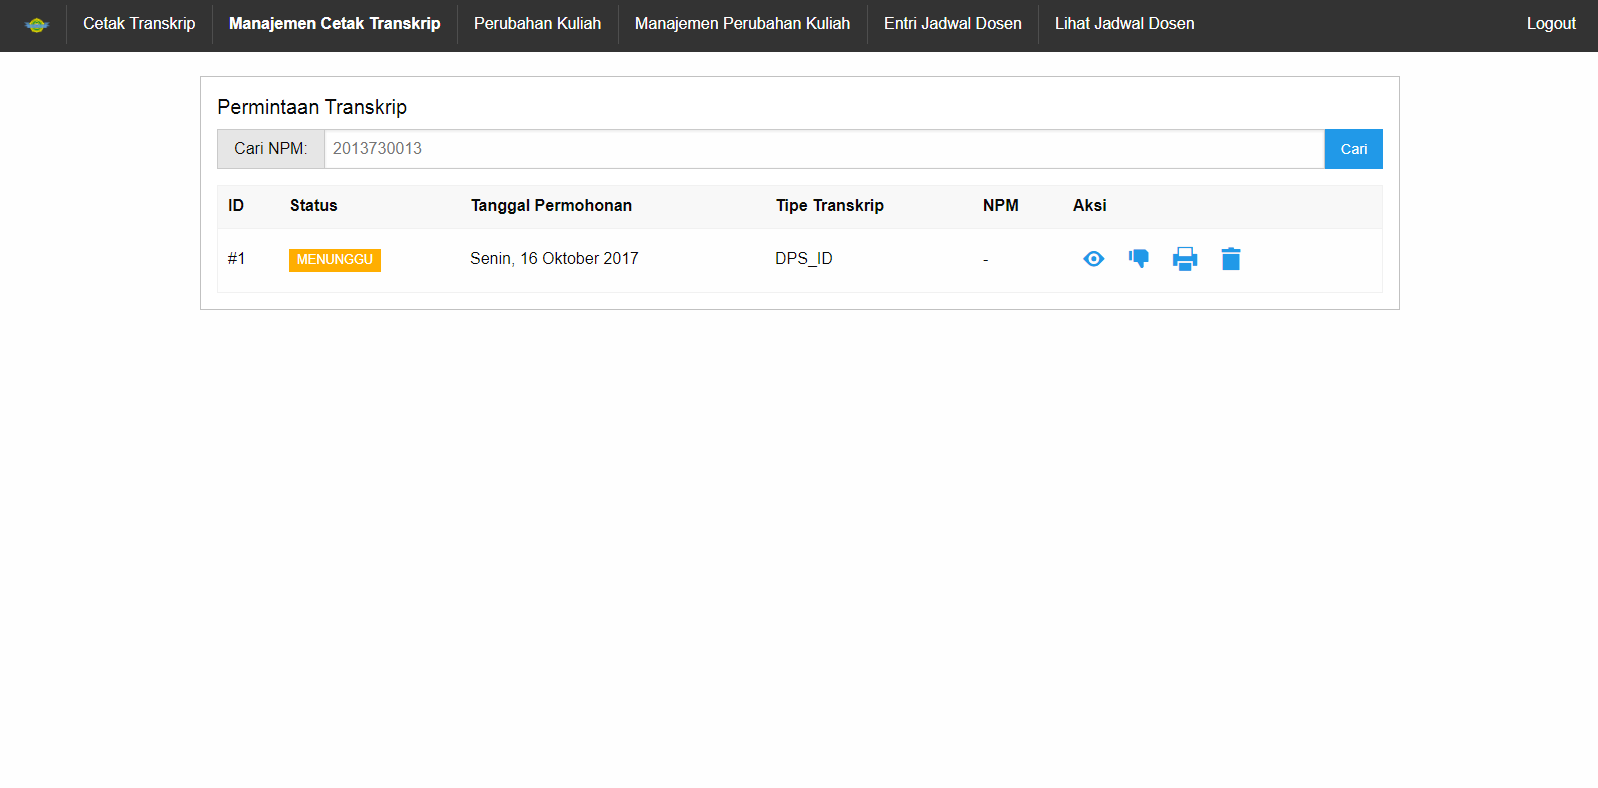
\includegraphics[scale=0.4]{manageTranskrip.png}}
	\caption[Tampilan Manajemen Transkrip]{Tampilan Manajemen Transkrip} 
\end{figure}
Untuk memohon pencetakan transkrip pada halaman tersebut mahasiswa diperlukan untuk melakukan :
\begin{enumerate}
  \item Memilih salah satu dari 3 tipe transkrip yang ada. Ada 3 tipe transkrip: Daftar Perkembangan Studi (DPS) Bahasa Inggris, DPS Bahasa Indonesia dan Lembar Hasil Studi Semester Akhir.
  \item Lalu mahasiswa mengisi keterangan keperluan pencetakan transkrip di \textit{field} keperluan.
  \item Setelah kedua hal tersebut dipilih dan diisi , tekan tombol "Kirim Permohonan" untuk memohon pencetakan transkrip ke Tata Usaha.
\end{enumerate}
Tata usaha memiliki beberapa opsi untuk merespon permintaan yang sudah dikirim mahasiswa tadi :
\begin{enumerate}
	\item Melihat detail permintaan transkrip
	\item Menolak permintaan transkrip
	\item Mencetak detail permintaan transkrip
	\item Menghapus permintaan transkrip
\end{enumerate}
\subsubsection{Struktur Kode Program}
\paragraph{}Kode program untuk modul \textit{Transcript Request / Manage} distruktur menggunakan struktur Model-View-Controller sebagai berikut:
\begin{itemize}
	\item Controller:
		\begin{itemize}
			\item TranskripManage.php: berfungsi untuk menghubungkan view dan model TranskripManage.
			\item TranskripRequest.php: berfungsi untuk menghubungkan view dan model TranskripRequest.
		\end{itemize}
	\item View:
		\begin{itemize}
			\item /TranskripManage/email.php: \textit{template} untuk email konfirmasi yang akan dikirim ke mahasiswa yang meminta transkrip.
			\item /TranskripManage/main.php: tampilan menu utama TranskripManage.
			\item /TranskripRequest/main.php: tampilan menu utama TranskripRequest.
			\item /TranskripRequest/email.php: \textit{template} untuk email pemberitahuan ke tata usaha bahwa ada mahasiswa yang meminta transkrip.
		\end{itemize}
	\item Model: Transkrip\_model.php: menghubungkan basis data tabel "transkrip" dengan modul. \textit{Transkrip Request/ Manage}
	\item \textit{Migration file}:
		\begin{itemize}
			\item 20160222153100\_Transkrip\_Initial.php: pembuatan tabel "transkrip".
			\item 20160513150200\_Transkrip\_TipeTranskrip.php: penambahan field \textit{requestType} di tabel "transkrip" dengan tipe \textit{varchar} berukuran 3.
			\item 20160520154600\_Transkrip\_BahasaTranskrip.php: mengubah ukuran field \textit{requestType} dari 3 menjadi 8.
		\end{itemize}
\end{itemize}

\subsection{Perubahan Kuliah}
\paragraph{} Perubahan kuliah adalah modul kedua yang sudah aktif di BlueTape. Modul ini berfungsi sebagai alat bagi staf UNPAR untuk mengirimkan permintaan perubahan kuliah ke karyawan tata usaha. Selain itu karyawan tata usaha juga dapat menggunakan modul ini untuk mengatur permintaan-permintaan yang sudah dikirim dari staf UNPAR tadi. 
\begin{figure} [H]
	\centering  
	\frame{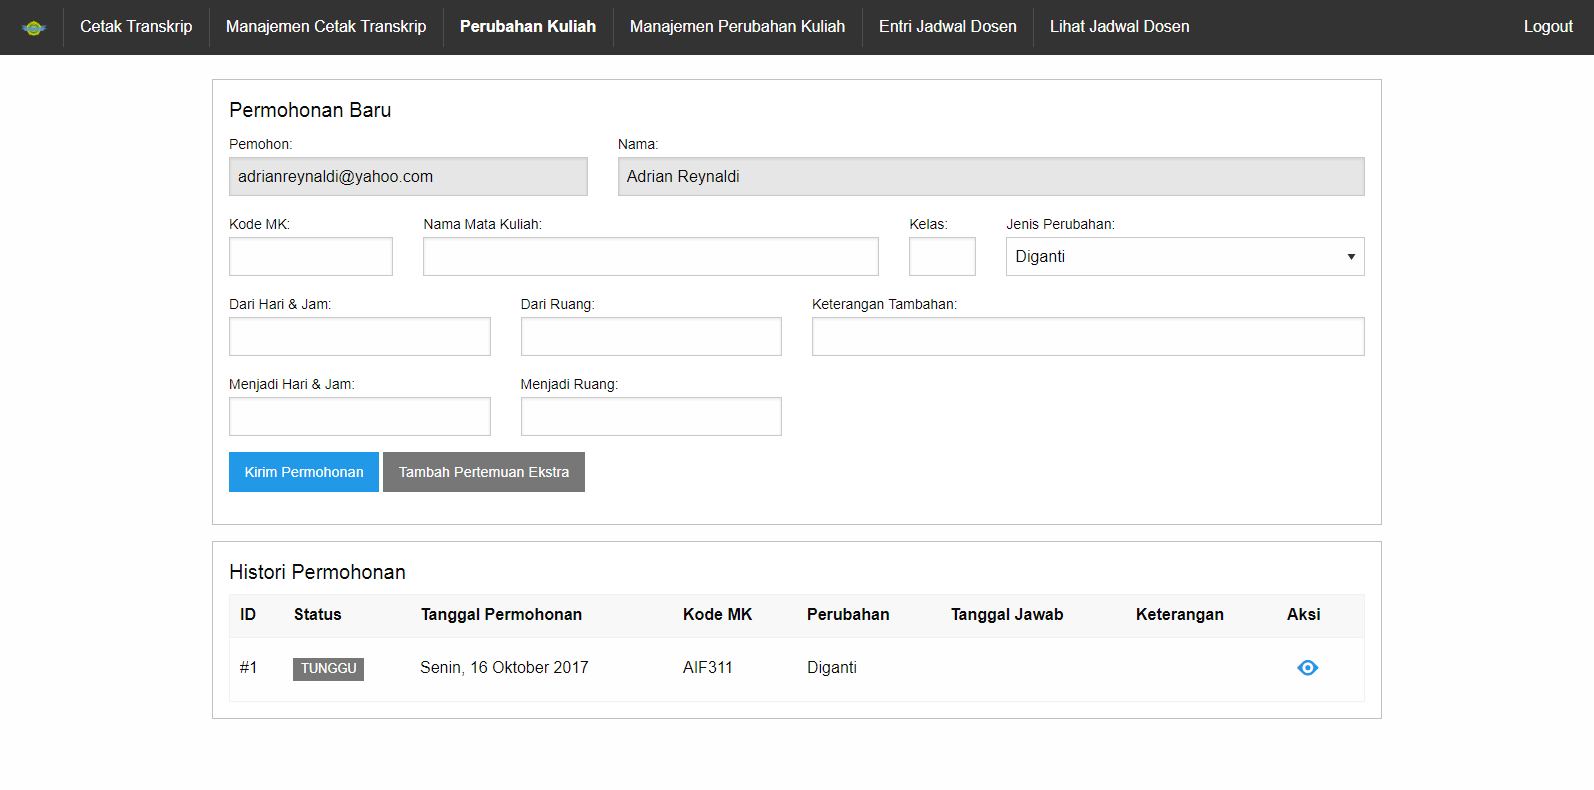
\includegraphics[scale=0.4]{perubahanKuliah.png}}
	\caption[Tampilan Menu Perubahan Kuliah]{Tampilan Menu Perubahan Kuliah} 
\end{figure}
\begin{figure} [H]
	\centering  
	\frame{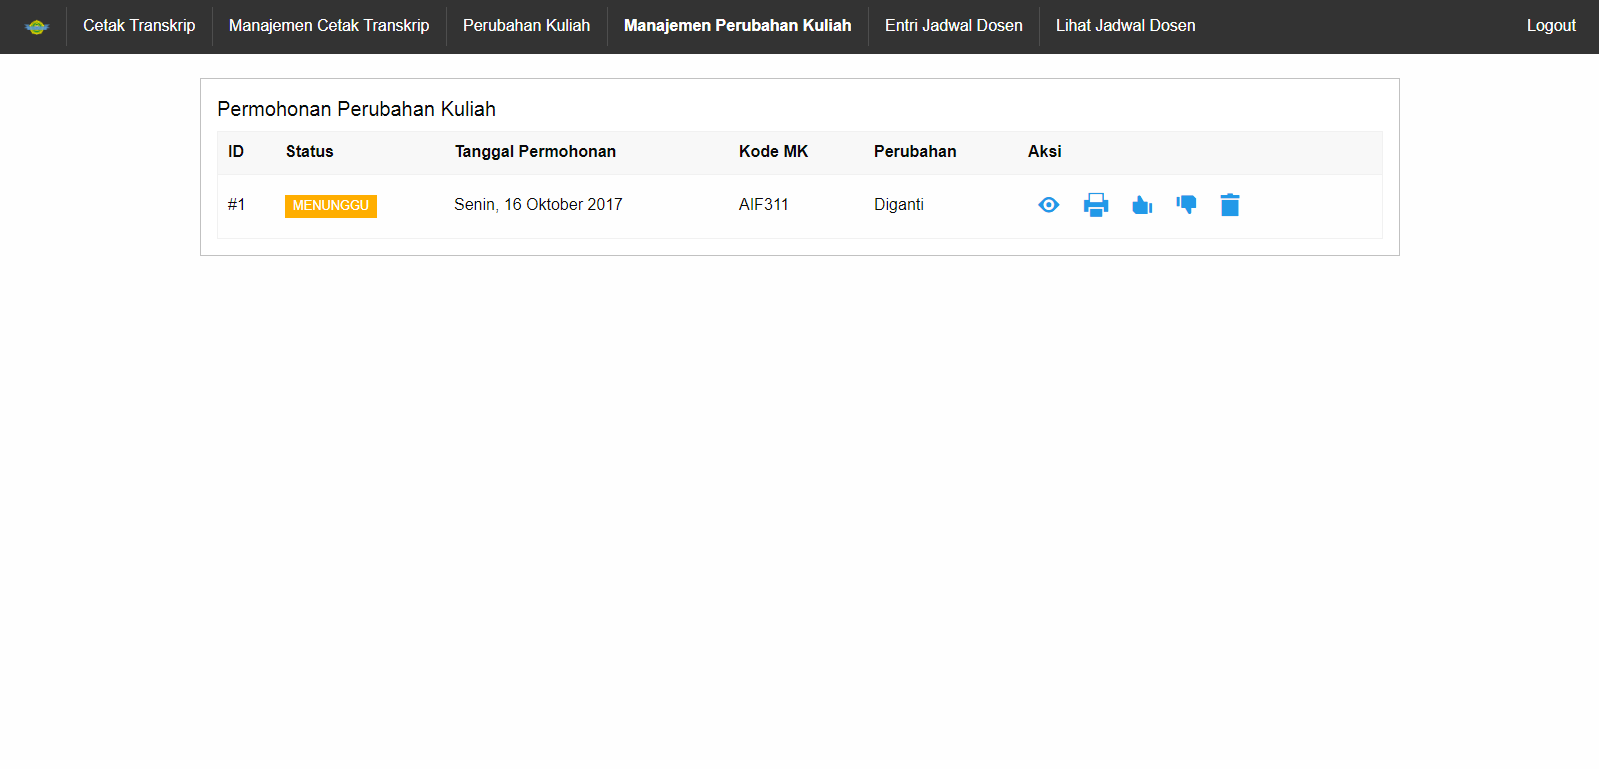
\includegraphics[scale=0.4]{managePerubahanKuliah.png}}
	\caption[Tampilan Menu Manajemen Perubahan Kuliah]{Tampilan Menu Manajemen Perubahan Kuliah} 
\end{figure}
Untuk membuat permintaan perubahan kuliah, staf UNPAR perlu mengisi setiap \textit{field} yang ada di menu. Setelah semua \textit{field} diisi, dosen bisa memilih untuk mengirim permohonan atau tambah pertemuan.
\begin{itemize}
	\item Tombol "Kirim Permohonan" akan memeriksa apakah data yang sudah dimasukan sudah benar, bila sudah maka data permohonan akan dikrim ke server dan apabila ada yang masih salah maka sistem akan menandai bagian yang salah.
	
	\item Tombol "Tambah Pertemuan Ekstra" akan memunculkan 2 \textit{field} baru yaitu \textit{field} "Menjadi Hari dan jam" dan \textit{field} "Menjadi Ruang". Bila dosen ingin mengirimkan permintaan penambahan pertemuan, tetap harus menekan tombol "Kirim Permohonan" setelah kedua \textit{field} yang baru tersebut juga diisi.
\end{itemize}
Di sisi tata usaha , modul ini memiliki fungsi untuk:
\begin{itemize}
	\item Menolak permintaan perubahan kuliah
	\item Menyetujui permintaan perubahan kuliah
	\item Mencetak detail perubahan kuliah
	\item Melihat detail perubahan kuliah
	\item Menghapus permintaan perubahan kuliah
\end{itemize}
 
\subsubsection{Struktur Kode Program}
\paragraph{}Kode program untuk modul Perubahan Kuliah distruktur menggunakan struktur Model-View-Controller sebagai berikut:
\begin{itemize}
	\item Controller:
		\begin{itemize}
			\item PerubahanKuliahManage.php: menghubungkan view dan model PerubahanKuliahManage.
			\item PerubahanKuliahRequest.php: menghubungkan view dan model PerubahanKuliahRequest.
		\end{itemize}
	\item View:
		\begin{itemize}
			\item /PerubahanKuliahManage/email.php: \textit{template} email konfirmasi ke pemohon perubahan kuliah.
			\item /PerubahanKuliahManage/main.php: tampilan menu utama PerubahanKuliahManage
			\item /PerubahanKuliahManage/printview.php: \textit{template} untuk membentuk file berisi data permohonan perubahan kuliah yang dapat dicetak oleh tata usaha.
			\item /PerubahanKuliahRequest/main.php: tampilan menu utama PerubahanKuliahRequest
			\item /PerubahanKuliahRequest/email.php: \textit{template} email pemberitahuan ke tata usaha bahwa ada yang memohon perubahan kuliah.
		\end{itemize}
	\item Model: PerubahanKuliah\_model.php: menghubungkan basis data dengan modul PerubahanKuliah
	\item \textit{Migration file}:
		\begin{itemize}
			\item 20161123123700\_PerubahanKuliah\_Initial.php: pembentukan tabel "perubahankuliah"
			\item 20170523125600\_PerubahanKuliah\_MultipleTo.php: \\
			File Migrasi ini berfungsi untuk beberapa hal:
				\begin{enumerate}
					\item menambah \textit{field} baru "to" di tabel "perubahankuliah" bertipe varchar dengan ukuran 1024 yang disimpan setelah field "toRoom".
					\item menghapus \textit{field} "toRoom".
					\item menghapus \textit{field} "toDateTime".
				\end{enumerate}
		\end{itemize}
\end{itemize}

\subsection{Golongan Pengguna Aplikasi}
Pada bagian ini akan dijelaskan pengelompokan tipe-tipe golongan pengguna aplikasi BlueTape yang diatur di file \textit{modules.php}.

\subsubsection{Mahasiswa FTIS}
Mahasiswa FTIS adalah semua mahasiswa Fakultas Teknologi Informasi dan Sains. Saat ini golongan Mahasiwa FTIS baru memiliki satu akses ke fitur untuk memnita transkrip.

\subsubsection{Tata Usaha UNPAR}
Tata Usaha UNPAR adalah golongan pengguna yang bekerja sebagai staff tata usaha di Universitas Katolik Parahyangan. Di BlueTape, Tata Usaha UNPAR memilki akses fitur-fitur sebagai berikut:
\begin{itemize}
	\item Mengatur permintaan transkrip dari mahasiswa
	\item Mengatur permintaan perubahan kuliah 
\end{itemize}

\subsubsection{Staf UNPAR}
Staf UNPAR adalah para pekerja dan karyawan di Universitas Katolik Parahyangan. Untuk saat ini golongan staf UNPAR hanya memiliki akses fitur untuk meminta perubahan kuliah.

\subsubsection{Mahasiswa Informatika}
Mahasiswa Informatika adalah pengguna yang memiliki kepentingan untuk mencetak transkrip nilai. Di Bluetape saat ini, Mahasiswa Informatika baru memiliki satu fitur yaitu untuk meminta transkrip nilai.


\subsection{Fitur Sistem Kini}
Untuk perincian fiturnya akan ditampilkan sebagai diagram usecase pada Gambar 3.6.
\begin{figure} [H]
	\centering  
	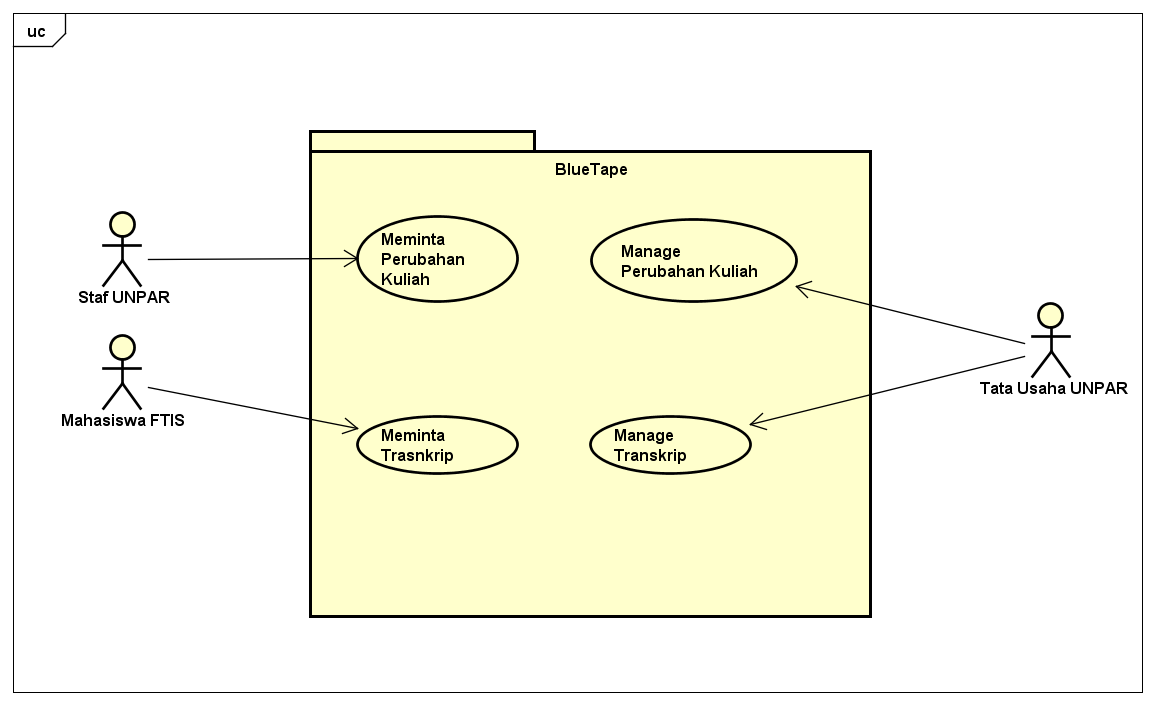
\includegraphics[scale=0.48]{useCaseDiagramAwal.png}
	\caption[Diagram Use Case Sistem Kini]{Diagram Use Case Sistem Kini} 
	\label{fig:flow-chart-CodeIgniter} 
\end{figure}

\section{Analisis Sistem Usulan: Aplikasi Pembangkit Jadwal Dosen}
Aplikasi Pembangkit Jadwal Dosen adalah aplikasi tambahan untuk BlueTape yang memiliki dua modul yaitu:
\begin{enumerate}
	\item Modul Entri Jadwal Dosen yang bisa melakukan:
		\begin{itemize}
			\item Input jadwal mingguan
			\item Mencatat update terakhir
			\item Ekspor jadwal ke XLS
		\end{itemize}
	\item Modul Lihat Jadwal Dosen yang bisa melakukan:
		\begin{itemize}
			\item Melihat jadwal-jadwal semua dosen
			\item Ekspor jadwal ke XLS
		\end{itemize}
\end{enumerate}
Langkah penggunaan program secara garis besarnya dapat dilihat pada Gambar 3.7
\begin{figure} [H]
	\centering  
	\includegraphics[scale=0.5]{chartPoster.png}
	\caption[Langkah Penggunaan Program]{Langkah Penggunaan Program} 
	\label{fig:flow-chart-CodeIgniter} 
\end{figure}
Keterangan langkah penggunaan:
\begin{enumerate}
	\item Pengguna login di BlueTape
	\item BlueTape mengotentikasi pengguna
	\item Jika email terdaftar pada list dosen, maka pengguna diberi akses ke EntriJadwalDosen dan LihatJadwalDosen
	\item Jika email menggunakan format 73xxyyyy@student.unpar.ac.id maka pengguna diberi akses ke modul LihatJadwalDosen saja.
\end{enumerate}
Untuk mengimplementasikan fitur-fitur tersebut maka digunakan teknologi:
\begin{itemize}
	\item PHP \& CodeIgniter
	\item Zurb Foundation
	\item Framework BlueTape
	\item Google OAuth
	\item PHPExcel
\end{itemize}

\subsection{Perancangan Basis Data}
Perancangan basis data dapat dilihat pada ER Diagram di Gambar 3.7
\begin{figure} [H]
	\centering  
	\includegraphics[scale=0.48]{ERD.png}
	\caption[ER Diagram Sistem Usulan]{ER Diagram Sistem Usulan} 
\end{figure}
Tabel bluetape\_userinfo dan jadwal\_dosen memiliki hubungan 1 ke n. 
Penjelaan setiap atribut pada jadwal\_dosen:
\begin{itemize}
	\item id merupakan primary key
	\item email merupakan foreign key yang merujuk ke atribut email di bluetape\_userinfo
	\item hari menyimpan hari dimulainya jadwal
	\item jam\_mulai menandakan waktu dimulainya jadwal
	\item jenis merupakan jenis jadwal
	\item label merupakan nama kegiatan jadwal
	\item update meruapakan waktu terakhir terjadi perubahan pada jadwal
\end{itemize}
\subsection{Fitur Sistem Usulan}
Untuk perincian fitur yang ditambahkan di BlueTape dapat dilihat pada diagram usecase di Gambar 3.8.
\begin{figure} [H]
	\centering  
	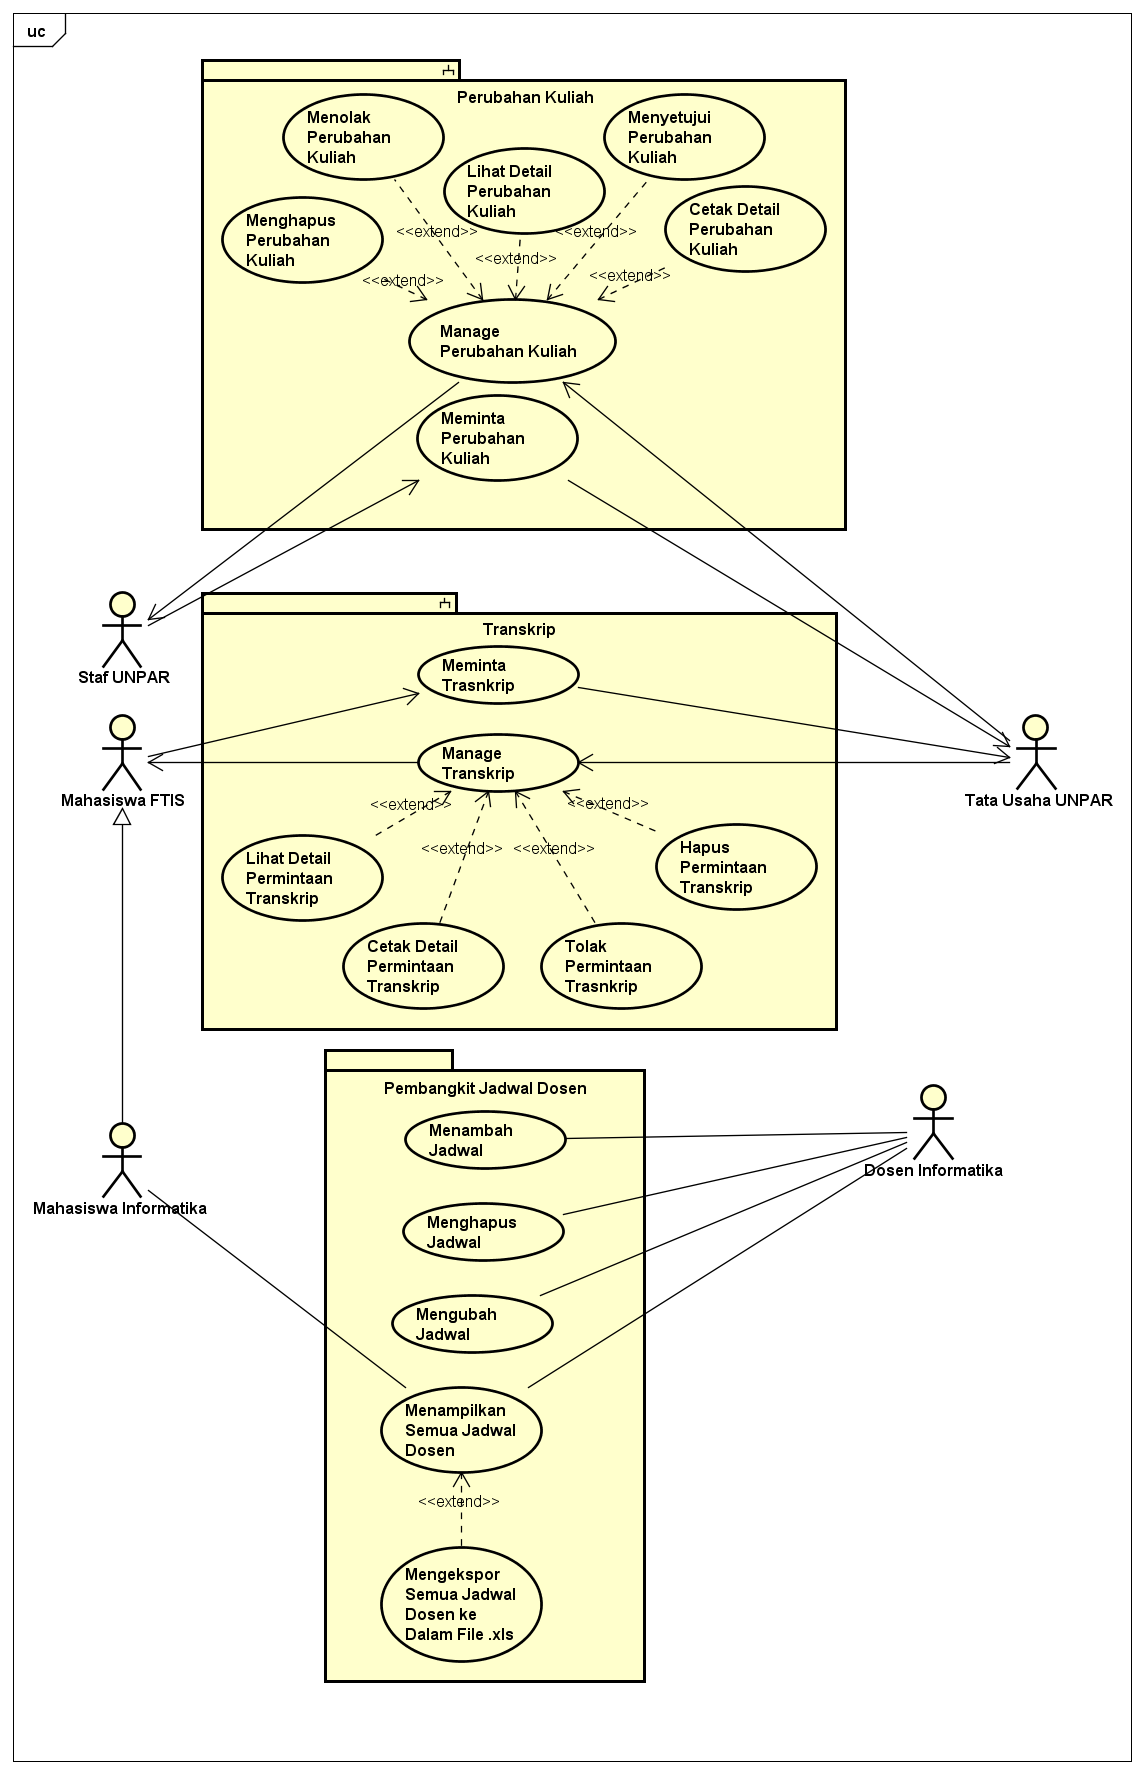
\includegraphics[scale=0.48]{useCaseDiagramSemua.png}
	\caption[Diagram Use Case Sistem Usulan]{Diagram Use Case Sistem Usulan} 
	\label{fig:flow-chart-CodeIgniter} 
\end{figure}

Tidak ada perubahan pada diagram \textit{usecase} dan skenario dari sistem kini (bisa dilihat pada Gambar 3.6) hanya ditambahkan bagian untuk Aplikasi Pembangkit Jadwal Dosen. Berikut ini adalah penjelasan skenario yang ditambahkan dari diagram \textit{usecase} pada Gambar 3.8:
\begin{enumerate}
	\item Skenario Menambah Jadwal
	\begin{itemize}
		\item Aktor: Dosen Informatika
		\item Skenario Normal
			\begin{enumerate}[1.]
				\item Dosen Informatika mengisi data jadwal
				\item Sistem menyimpan data jadwal tersebut ke dalam \textit{database}
			\end{enumerate}
	\end{itemize}

	\item Skenario Mengubah Jadwal
	\begin{itemize}
		\item Aktor: Dosen Informatika
		\item Skenario Normal
			\begin{enumerate}[1.]
				\item Dosen Informatika memilih jadwal yang akan diubah
				\item Sistem menampilkan menu pengubahan berisi data jadwal yang dipilih tadi
				\item Dosen Informatika mengubah data yang ingin diubah
				\item Sistem menyimpan hasil perubahan ke dalam database
			\end{enumerate}
	\end{itemize}


	\item Skenario Menghapus Jadwal
	\begin{itemize}
		\item Aktor: Dosen Informatika
		\item Skenario Normal
			\begin{enumerate}[1.]
				\item Dosen Informatika memilih jadwal yang akan dihapus
				\item Sistem menampilkan menu pengubahan berisi data jadwal yang dipilih
				\item Dosen Informatika menekan tombol hapus
				\item Sistem menghapus data jadwal tersebut yang ada di database
			\end{enumerate}
	\end{itemize}

	\item Skenario Menampilkan Semua Jadwal Dosen
	\begin{itemize}
		\item Aktor: Mahasiswa Informatika, Dosen Informatika
		\item Skenario Normal
			\begin{enumerate}[1.]
				\item Aktor memilih menu lihat jadwal dosen
				\item Sistem memuat semua data jadwal-jadwal dari \textit{database}
				\item Sistem mengelompokan setiap jadwal berdasarkan pemiliknya
				\item Sistem membuat tab-tab yang merepresentasikan setiap dosen yang sudah menyimpan jadwal ke dalam database
				\item Sistem memasukan jadwal-jadwal ke dalam tab-tab sesuai nama pemiliknya.
			\end{enumerate}
	\end{itemize}
	

	\item Skenario Mengekspor Semua Jadwal Dosen ke Dalam File .xls
	\begin{itemize}
		\item Aktor: Mahasiswa Informatika, Dosen Informatika
		\item Skenario Normal
			\begin{enumerate}[1.]
				\item Aktor memilih menu lihat jadwal dosen
				\item Sistem memuat semua data jadwal-jadwal dari \textit{database}
				\item Sistem mengelompokan setiap jadwal berdasarkan pemiliknya
				\item Sistem membuat tab-tab yang merepresentasikan setiap dosen yang sudah menyimpan jadwal ke dalam database
				\item Sistem memasukan jadwal-jadwal ke dalam tab-tab sesuai nama pemiliknya.
				\item Aktor menekan tombol ekspor
				\item Sistem mengkonversi semua data jadwal dari bentuk php ke dalam bentuk \textit{spreadsheet} .xls
				\item Sistem menampilkan menu pemilihan lokasi penyimpanan \textit{file} .xls
				\item Aktor menekan tombol simpan
				\item Sistem menyimpan file .xls tersebut di lokasi yang sudah dipilih oleh aktor.
			\end{enumerate}
		\item Skenario Exception
			\begin{enumerate}[1.]
				\item Aktor memilih menu lihat jadwal dosen
				\item Sistem memuat semua data jadwal-jadwal dari \textit{database}
				\item Sistem tidak menerima data apapun dari \textit{database}
				\item Sistem men-\textit{disable} tombol ekspor
			\end{enumerate}
	\end{itemize}
\end{enumerate}

\subsection{Pengguna Aplikasi}
Pada bagian ini akan dijelaskan pengelompokan tipe-tipe pengguna aplikasi BlueTape dengan sistem usulan. Perubahan terjadi pada kelompok "Mahasiswa Informatika" yang mendapat fitur tambahan. Selain itu , ada penambahan kelompok pengguna yaitu "Dosen Informatika". Perubahan-perubahan akan dijelaskan pada bagian masing-masing.

\subsubsection{Mahasiswa FTIS}
Mahasiswa FTIS adalah semua mahasiswa Fakultas Teknologi Informasi dan Sains. Saat ini golongan Mahasiwa FTIS baru memiliki satu akses yaitu untuk memnita transkrip.


\subsubsection{Tata Usaha UNPAR}
Tata Usaha UNPAR adalah golongan pengguna yang bekerja sebagai staff tata usaha di Universitas Katolik Parahyangan. Di BlueTape, Tata Usaha UNPAR memilki akses fitur-fitur sebagai berikut:
\begin{itemize}
	\item Mengatur permintaan transkrip dari mahasiswa
	\item Mengatur permintaan perubahan kuliah 
\end{itemize}

\subsubsection{Staf UNPAR}
Staf UNPAR adalah para pekerja dan karyawan di Universitas Katolik Parahyangan. Untuk saat ini golongan staf UNPAR hanya memiliki akses fitur untuk meminta perubahan kuliah.

\subsubsection{Mahasiswa Informatika}
Mahasiswa Informatika adalah semua mahasiswa jurusan Informatika di FTIS. Mahasiswa informatika memiliki akses pada beberapa fitur sebagai berikut:
\begin{itemize}
	\item Melihat semua jadwal dosen Informatika
	\item Mengekspor semua jadwal dosen Informatika ke dalam tipe file .xls
	\item Meminta transkrip nilai
\end{itemize}

\subsubsection{Dosen Informatika}
Dosen merupakan pengguna yang dapat memasukan jadwal-jadwalnya ke dalam BlueTape agar dapat dilihat mahasiswa. Dosen memilki akses pada fitur:
\begin{itemize}
	\item Memasukan jadwal ke dalam BlueTape
	\item Mengubah jadwal yang sudah dimasukan  
	\item Menghapus jadwal yang sudah dimasukan
	\item Melihat semua jadwal dosen , termasuk jadwal miliknya sendiri
	\item Mengeskpor semua jadwal dosen ke dalam tipe file .xls
\end{itemize}